\section{Auswahl und Beschreibung der Messmethode}
\label{chap:auswahl_beschreibung_methode}

Während die CPU ein Programm ausführt, das aus einer Reihe von Befehlssätzen besteht, verbraucht er unterschiedlich viel Strom. Die Idee der hier erstellten Messmethode ist es, ein Programm kontrolliert und mit präzis ausgewählten Befehlssätzen auf der CPU durchlaufen zu lassen. Das Programm in Form eines Benchmarks ist so konzipiert, dass ein bestimmter Befehlssatz millionenfach wiederholt wird. Dadurch wird der Stromverbrauch während der Ausführung über einen längeren Zeitraum konstant gehalten. Denn nur so ist eine aussagekräftige Messung möglich, da ein einzelner Befehlssatz so schnell durchläuft, dass er kaum messbar wäre. Da die Ausführung der Befehlssätze wiederholt wird, muss die Messung durch die Anzahl der ausgeführten Wiederholungen geteilt werden.
\par
Die Strommessung erfolgt vom Leistungsverbrauch des ganzen Gerätes. Optimal wäre es, nur die Leistung der CPU zu messen. Dafür müsste aber die CPU vom Board ausgelötet werden und eine speziell dafür gebaute Messvorrichtung verwendet werden. Dazu kommt, dass nicht alle Datenblätter, welche die erforderliche Beschreibung und Belegung der Pins enthalten, für jedes Board oder für jeden Chip verfügbar sind. Deshalb wird ein SoC eingesetzt und die gesamte Leistung gemessen. SoC sind verfügbar auf kleinen Entwickler-Boards, die keine Lüfter, Laufwerke oder andere Verbraucher aufweisen, die hinsichtlich der Leistung störende Unregelmässigkeiten verursachen würden.



\begin{wrapfigure}{R}{0.6\textwidth}
\centering
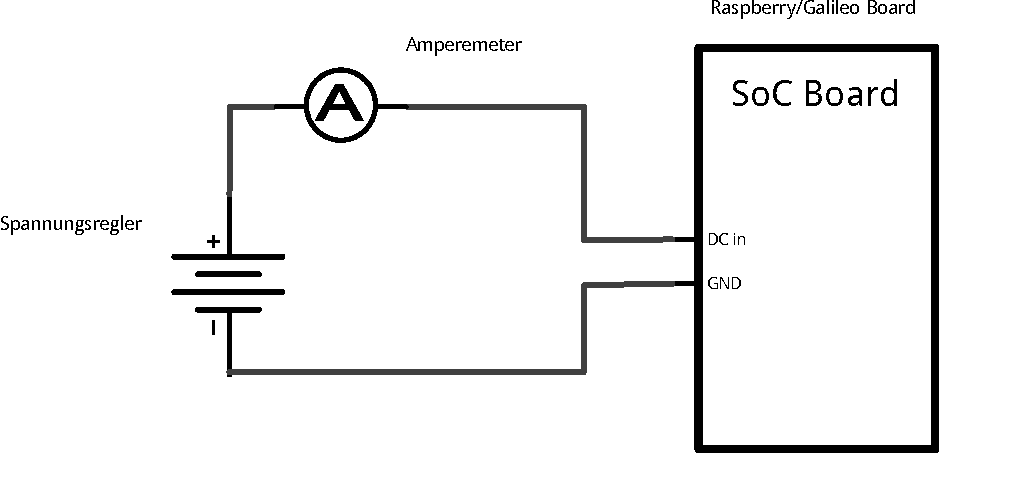
\includegraphics[scale=0.5]{images/schema.pdf}
\caption{Elektroschema für die Messung}
\label{fig:Elektroschema}
\end{wrapfigure}


Die für diese Arbeit verwendeten Boards werden im nächsten Kapitel \autoref{beschreibung_hardware} beschrieben. Es wird davon ausgegangen, dass während der Durchführung des Benchmarks, die Komponenten auf dem Board abgesehen vom CPU selbst, vernachlässigbar kleine Leistungsschwankungen aufweisen. Die Messung erhält somit eine Grundleistung, die vom Resultat abgezogen werden muss. Die Speisung erfolgt über einen Spannungsregler, der der Schaltung eine konstante Spannung liefert. Zwischen dem Spannungsregler und der Schaltung ist ein Amperemeter (Multimeter) zwischengeschaltet, der die Messung vornimmt. In der Abbildung \ref{fig:Elektroschema} ist das Elektroschema und die Platzierung des Amperemeters ersichtlich.
\par
Der eigentliche Kern des Benchmarks besteht aus gezielten und kurzen Assembler-Zeilen. Der Assemblercode bewirkt eine Schleife über einen zu testenden Befehlssatz. Damit das Ergebnis über einen längeren Zeitraum gemessen werden kann, wird die Schleife in einer Grössenordnung von 100 Millionen nacheinander wiederholt. Dies erstellt für die Messung einen Zeitraum von ca. einer halben Minute auf einem 800MHz CISC-Prozessor.
\par
Während dem Durchlaufen des Benchmarks darf die Ausführung nicht gestört werden. Jedes moderne Betriebssystem ist multitaskingfähig. Das bedeutet, dass das Betriebssystem eine Zeitscheibe besitzt und die Ressourcen des CPUs abwechslungsweise an die Prozesse verteilt werden. Ein Benchmark darf also nicht als gewöhnlicher Prozess von einem Betriebssystem gestartet werden. Würde man das tun, hätte man keine Kontrolle, wann und wieviele Ressourcen der Benchmark schlussendlich zugesprochen bekommt. Diese mangelnde Kontrolle würde das Messresultat verfälschen. Im Rahmen dieser Arbeit musste eine Methode erarbeitet werden, damit der Benchmark während der Durchführung die vollen Ressourcen der CPU bekommt und somit ein kontrollierter Ablauf garantiert ist.
\par
Die Ursprungsidee war es, direkt auf Baremetal zu arbeiten. Baremetal ist eine Ausdruck dafür, dass direkt auf der Hardware gearbeitet wird. Bei dieser Methode wird auf ein Betriebssystem verzichtet. Nach dem Bootprozess der Hardware wird direkt ein Programm gestartet und ausgeführt. An dieser Stelle käme der Benchmark zum Zug. Eine speziell dafür präparierte Partition mit dem Benchmark würde die Hardware booten und den Benchmark ausführen.
\par
Für die Baremetal-Methode wurde ein funktionstüchtiger Prototyp erstellt. Es zeigten sich aber einige Nachteile. Auf komplexerer Hardware mit x86-Prozessoren ist der Boot-Vorgang um ein Vielfaches aufwändiger\cite{intel_boot_process}. Diese Prozessoren-Typen können nicht einfach beim Einschalten einen Programmcode ausführen. Es muss vorher eine lange Reihe von Abläufen in der Preboot Phase berücksichtigt und ausgeführt werden. Als zweiter Nachteil der Baremetal-Methode ist die Überprüfung des Benchmarks. Um sicherzustellen, dass der Benchmark erwartungsgemäss funktioniert oder überhaupt die Feststellung, dass er ausgeführt wird, benötigt ein Feedback nach aussen. Eine LED-Leuchte würde für dieses Feedback bereits ausreichen. Die GPIOs, die nötig sind, um das LED zu steuern, sind je nach SoC sehr schwierig anzusprechen, weil sie über einen PCI-Bus verbunden sind. Das Betriebssystem stellt normalerweise die nötigen C-Libraries zur Verfügung, um die Komponenten, wie die GPIO, über einen PCI-Bus anzusteuern. Der dritte Nachteil auf einer Methode, ohne Betriebssystem zu arbeiten, ist die aufwändige Vorbereitung jedes einzelnen Tests. Für jeden Test muss eine Partition mit dem Benchmark erstellt und auf ein Medium kopiert werden. Die Hardware muss neu gestartet werden,
damit die Messung erfolgen kann. Unter diesen Umständen wird ein automatisierter Betrieb erheblich erschwert.
\par
Wegen der oben genannten Nachteile, wurde ein neues Konzept ausgearbeitet. Das neue Konzept arbeitet auf Linux und bringt dadurch die Vorteile eines Betriebssystem mit sich. Es muss sicher gestellt werden, dass der Benchmark ohne Unterbrüche und abgeschirmt von anderen Prozessen durchgeführt werden kann. Um dies zu erreichen, wird der Benchmark anstelle des Benutzermodus (engl. User Space) im Kernelmodus (engl. Kernel Space) ausgeführt\cite{Mandl2010}. Ein Programm, das innerhalb des Kernelmodus ausgeführt wird, muss als Kernelmodul kompiliert und angemeldet werden. Schlussendlich kann nur ein Interrupt das Programm starten. Die genaue Beschreibung ist im \autoref{chap:benchmark_basis_interrupts} aufgeführt. Durch die Ausführung des Benchmark werden alle Prozesse, die auf dem Betriebssystem parallel ausgeführt werden gestoppt und der Benchmark bekommt die vollen CPU-Ressourcen zugesprochen. In ein Kernelmodul können unterschiedliche Benchmarks gleichzeitig hinein kompiliert werden. Somit wird die Ausführung unterschiedlicher Tests vereinfacht. Durch eine zusätzliche Automatisation würde ebenfalls die Messung erleichtert. 

 



 
